
\section{Computer Use Datasets}\label{sec:datasets}
In this section, we focus on important computer use datasets and do not cover datasets used for general pre-training of foundation models or those only partially relevant for computer use, such as question answering \citepeg{hudson2019gqa} and tool usage datasets \citepeg{patil2023gorilla}.
\Cref{tab:overview_datasets} provides an overview of all considered computer use datasets and their key properties.

To illustrate the evolution of these datasets, \Cref{fig:dataset-timeline} presents a timeline of their development across three major domains: Web, Android, and personal computers. The figure reflects a general trend toward increasing task complexity and realism over time, highlighting how research has shifted from simplified environments toward real-world applications and large-scale demonstrations.


\begin{figure}[t]
    \centering
    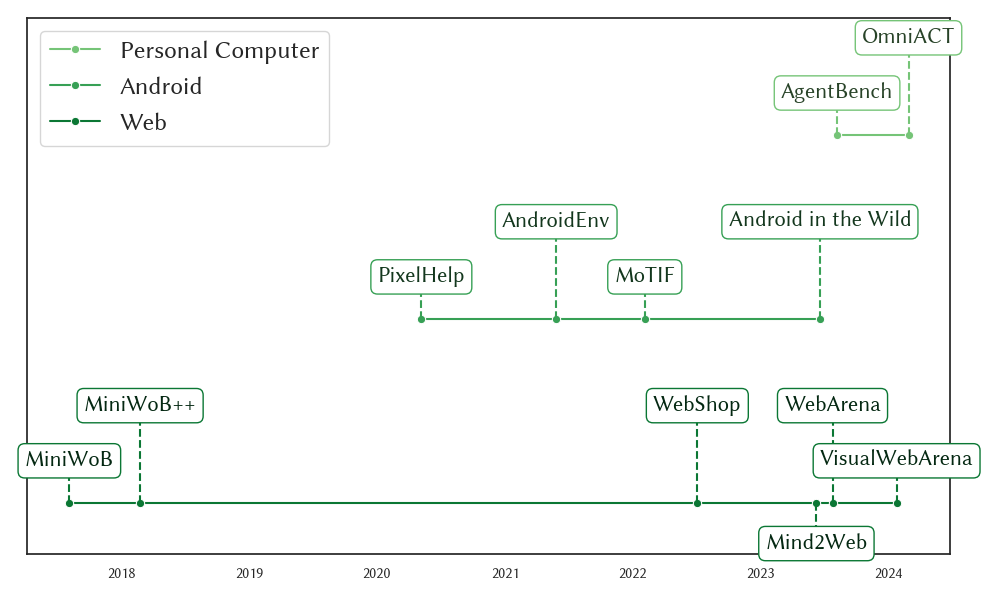
\includegraphics[width=0.7\linewidth]{figures/dataset_domain_timeline.png}
    \caption{Development of datasets across domains over time. In general, complexity increases over time. For the \emph{Web domain}: MiniWoB \citep{shi_world_2017} and MiniWoB++ \citep{liu_reinforcement_2018} contain $100$ tasks on a simplified UI. WebShop \citep{yao_webshop_2022} is a more realistic single webshop application focusing on realistic product diversity. Mind2Web \citep{deng_mind2web_2023} contains $2350$ demonstrations across $137$ actual websites. WebArena \citep{zhou_webarena_2024} is a controlled environment of $4$ realistic web applications. VisualWebArena \citep{koh_visualwebarena_2024} extends WebArena with $910$ more visual tasks and an additional application. For the \emph{Android domain}: PixelHelp \citep{li_mapping_2020} contains step-by-step instructions across $4$ applications. AndroidEnv \citep{toyama_androidenv_2021} provides a framework to define custom tasks in Android applications. MoTIF \citep{avidan_dataset_2022} contains $756$ demonstrations across 125 applications. Android in the Wild \citep{rawles_android_2023} provides over $700,000$ demonstrations across $357$ applications. For the \emph{personal computer domain}: AgentBench \citep{liu_agentbench_2023-1} is a benchmark framework that spans operating systems, databases, web, and gaming tasks, including existing benchmarks like WebShop or Mind2Web. OmniACT \citep{kapoor_omniact_2024} contains $9802$ tasks labeled with straight-line code actions spanning $57$ applications on Windows, MacOS, Linux, and the Web.}
    \Description{The figure shows the chronological order of dataset releases for Web, Android, and Personal Computer domains over the years 2017 to 2024. It reveals that the Web domain saw earlier development activity, starting in 2017, while large-scale Android and Personal Computer datasets began emerging around 2020 and 2023, respectively. The timeline also indicates a concentration of new datasets in 2023 and 2024 across all domains, suggesting recent intensified interest. Although dataset complexity is not visually encoded, the temporal arrangement highlights the evolving landscape of task diversity and domain coverage over time.}
    \label{fig:dataset-timeline}
\end{figure}

\subsection{Dataset Types}
% Computer use datasets must fulfill two properties:
% \begin{itemize}
%     \item \textbf{Teaching Signal:}  The dataset must provide a teaching signal, enabling the agent to receive feedback on its actions $a_t$ or trajectories $\tau$, which is essential for guiding the learning process.
%     \item \textbf{Isolated Execution:} Training is typically conducted offline, separate from the final deployment platform, to prevent the agent from executing tasks that could have real-world consequences, such as modifying production databases or booking flight tickets during the learning phase.
%\end{itemize}

ACUs leverage two types of computer use datasets:
%

\begin{description}
    \item[Controlled Environments:] 
    A controlled environment is a simulated setting, meaning an agent can act freely without consequences, as the simulation can always be reset.
    These environments support reinforcement learning, given they provide an additional reward signal  \citepeg{humphreys_data-driven_2022}.
    Furthermore, they can be utilized to collect long-term memories in a safe simulation phase \citepeg{wen_autodroid_2024} and to plan at inference time by simulating potential actions \citep{koh_tree_2024}.
    \item[Offline Dataset: ]
    An offline dataset is collected by instructing humans on a computer task while recording observations and executed actions.
    The agent only sees the recorded interaction during training, meaning it never acts in the underlying environment, making training safe from consequences.
    % Collecting human trajectories is more straightforward than creating a controlled environment.
    Offline datasets can be utilized for few-shot learning \citepeg{deng_mind2web_2023} or fine-tuning an agent \citepeg{rahman_v-zen_2024} in an uncontrolled environment like a productive website. Furthermore, an offline dataset of a controlled environment can be used for initial behavioral cloning to combat sparse rewards \citep{humphreys_data-driven_2022}.
\end{description}

Both dataset types have distinct characteristics. 
Controlled environments are costly to create because they involve engineering simulations that mimic real-world behaviors, but the agent can explore all aspects of the environment autonomously.
In contrast, offline datasets can be recorded in any environment, but are incomplete as not every possible interaction is captured.
Furthermore, offline datasets only show a single trajectory to achieve an instruction, but maybe multiple ones exist.


\subsection{Domains, Observation and Action Spaces}
By analyzing the domains of our $\numdatasets$ reviewed datasets, we find that the majority of existing datasets are from the Web domain \citepeg{zhou_webarena_2024} and Android domain \citepeg{rawles_android_2023}, while the personal computer domain \citepeg{hong_cogagent_2024} receives less attention (see Appendix~\cref{fig:dataset-domain-dist}).

The types of observations and actions available in these datasets vary depending on the domain and data collection method. For observations, some datasets provide only image screen representations \citepeg{rawles_android_2023}, some only textual screen representations \citepeg{pasupat_mapping_2018}, while others offer both \citepeg{chen_websrc_2021}. Regarding actions, some datasets focus solely on mouse/touch and keyboard actions \citepeg{kapoor_omniact_2024}, some provide direct UI actions \citepeg{chen_webvln_2024}, while others focus on task-tailored actions \citepeg{liu_agentbench_2023}.
\Cref{tab:overview_datasets} provides an overview.
% Executable code is generally absent from offline datasets, as it is not feasible to record all possible code snippets an agent could generate.
% 
In many cases, additional observation and action types can be generated through post-processing efforts. For instance, HTML representations can be rendered through a web browser to provide image-based screen representations.

\subsection{Dataset Complexity}
Several factors, including the size of the state, observation, and action spaces, and the diversity of the tasks, influence the complexity of a computer use dataset. 
%These factors vary significantly between controlled environments and offline datasets.

Controlled environments are often simplified and less diverse compared to offline datasets. 
For instance, in MiniWoB++ \citep{shi_world_2017}, all tasks are performed within a uniform, simplified website design with minimal graphical user interface (GUI) elements and clean HTML. 
Similarly, WebShop \citep{yao_webshop_2022} is limited to a single, simplified webshop application. 
While WebArena \citep{zhou_webarena_2024} offers more realistic web environments, it is limited to four tasks.

Offline datasets tend to feature more realistic observations, with the diversity depending on the variety of scenarios, such as how many websites were included.
For example, Mind2Web \citep{deng_mind2web_2023} records tasks from 137 websites across 31 categories, providing substantial diversity.
Similarly, Android in the Wild \citep{zhang_android_2024} records tasks spanning 357 Android apps or websites.
% Offline datasets collected within controlled environments inherit the simplicity of the controlled environment, limiting their complexity and diversity.

The complexity of tasks varies greatly across datasets. 
For example, MiniWoB++ \citep{shi_world_2017} includes 100 tasks with randomized text and an average of 3.6 actions per task, ranging from simple actions like clicking a button to more complex tasks like filling out a form to book a flight. 
WebShop \citep{yao_webshop_2022} offers 12,000 crowd-sourced instructions, all related to shopping, with an average of 11.3 actions per task. 
Mind2Web \citep{deng_mind2web_2023} provides 2,000 tasks averaging 7.3 actions, while WebArena \citep{zhou_webarena_2024} features 812 tasks, some requiring actions across applications, such as the task to create a Reddit account mirroring a GitLab profile.

Generally, the complexity of newer datasets increases as agents become more capable.
A straightforward way to do this is to make observations and tasks more diverse and challenging.
For example, WebArena \citep{zhou_webarena_2024} has a more realistic observation space than MiniWoB++ \citep{shi_world_2017}, and tasks require more actions to be achieved.
However, there are many other ways to increase complexity:
VisualWebArena \citep{koh_visualwebarena_2024} adds images as part of the instruction, such as asking an agent to create a post selling a product shown in an image.
%\texttt{Help me make a post selling this item and navigate to it. Price it \$10 cheaper than the most similar item on the site}. 
AgentStudio \citep{zheng_agentstudio_2024} provides video-based observations, requiring agents to process dynamic, time-dependent information. 
MT-Mind2Web \citep{deng_multi-turn_2024} extends Mind2Web by introducing multi-turn tasks, where users give sequential instructions to the agent, requiring a more nuanced agent behavior.
MoTIF \citep{avidan_dataset_2022} introduces infeasible instructions in its offline dataset, challenging agents to recognize unachievable tasks.

\subsection{Recommendations}
\begin{comment}
A key limitation of current datasets lies in their insufficient task complexity, with most tasks within existing datasets involving a limited number of actions (averaging fewer than 10).
While increasing the number of actions can contribute to complexity, a more significant factor lies in the nature of these actions.
Actions can causally depend on previous actions, increasing task complexity.
For example, a meeting suggestion based on availability can only occur \emph{after} looking up available time slots.
In contrast, some actions can be performed in any order, such as filling out form fields, which typically indicates their independence from one another.
As such, we recommend that \textbf{future ACU datasets to increase the task complexity by requiring more actions, specifically causally dependent actions}.
\end{comment}


A key limitation of current datasets lies in their insufficient trajectory complexity. They have limited structural and causal dependencies between actions in a task sequence. Complex tasks often require agents to execute actions in a specific causal order, where later actions depend on the outcomes of earlier ones. For instance, proposing a meeting time requires first retrieving the user's availability. In contrast, filling form fields can often be performed in any sequence. We recommend that \textbf{future ACU datasets increase trajectory complexity} by designing tasks that require longer, causally dependent action sequences.

Although trajectory complexity is crucial, observation, action, and task diversity should not be neglected, as broader observation and action types (e.g., dealing with various UI components) and more diverse tasks within and across applications are essential for accurately reflecting real-world usage and improving the generality of agents.
